\section{Настройка и управление параметрами ЭА.}

\begin{itemize}
    \item Параметры надо выбирать обоснованно, т.к. плохой выбор может привести к сильному ухудшению времени работы. Параметры подобранные эмпирическим путем априори не будут оптимальными.
    \item Иногда нужно настраивать параметры в процессе работы!
\end{itemize}

\textbf{Настройка параметров}
Пример постановки задачи
\begin{itemize}
    \item Задачи: линейные псевдобулевы функции на битовых строках длиной n 
    \item Эволюционный алгоритм: (1 + 1)-ЭА, вероятность мутации бита: c/n
\end{itemize}

Известные результаты
\begin{itemize}
    \item c = 1: оптимальное время работы (для данного класса): $(e ± o(1)) · n ln n $
    \item c < 1: плавное ухудшение времени работы: $( \frac{e^c}{c} ± o(1)) · n ln n$
    \item c > 1, $OnEMax$ : плавное ухудшение времени работы (та же формула)
    \item c > 16, некоторые линейные функции: \textbf{экспоненциальное} время работы! 
\end{itemize}


\textbf{Управление параметрами}
Пример постановки задачи
\begin{itemize}
    \item Задача: $LEADIngOnES$: длина префикса из единиц в битовой строке длиной n 
    \item Эволюционный алгоритм: (1 + 1)-ЭА, вероятность мутации бита: $p$
\end{itemize}

Известные результаты
\begin{itemize}
    \item $p = 1/n: \frac{e-1}{2} n^2 ± O(n) ≈ 0.86n^2$
    \item $p = (1.59...)/n: ≈ 0.77n^2$
    \item Выбор p наилучшим образом в зависимости от приспособленности: \textbf{$≈ 0.68n^2$}
    \item Выбор p \textbf{динамически} в зависимости от факта улучшения: \textbf{$≈ 0.68n^2$}
\end{itemize}


\textbf{Методы управления параметрами:}
\begin{itemize}
    \item Правило "одной пятой" (один из вариантов)
    \begin{itemize}
        \item Рассматриваем (1 + 1)-ЭА
        \item Два гиперпараметра: $F > 1$ и $s$, управляем вероятностью мутации $p$
        \item Правило в общем виде:
        \begin{itemize}
            \item Потомок не хуже родителя: $p ← p · F$ 
            \item Потомок хуже родителя: $p ← p/F^{1/s}$
        \end{itemize}
        \item «Правило одной пятой»: $s= 4, F ≈ 1.5$
        \begin{itemize}
            \item Стремится к тому, чтобы на одно улучшение приходилось $s$ итераций без улучшения. Тогда улучшение будет один раз в $s + 1$ итераций
        \end{itemize}
        \item «Правило 1/e: $s= e-1, F = 1 + \frac{(logn)^2}{n}$ (\textbf{для F нужно уже другое значение})
    \end{itemize}
    \item 2-rate
    \begin{itemize}
        \item Для алгоритмов с дочерними популяциями, например, (1 + λ)-ЭА 
        \item Поддерживаем вероятность мутации $p$ в пределах от $p_{min}$ до $1/2$
        \item На каждой итерации:
        \begin{itemize}
            \item Половину потомков создаем с вероятностью мутации $2p$
            \item Половину потомков создаем с вероятностью мутации $p/2$
            \item Пусть $p′$ — вероятность мутации, с которой был сгенерирован лучший потомок
            \begin{itemize}
                \item С вероятностью $1/2$ устанавливаем $p ← p′$
                \item Иначе меняем случайным образом или на $2p$, или на $p/2$
            \end{itemize}
        \end{itemize}
        \item Применяем ограничение: $p ← min(1/2, max(p_{min}, p ))$
        \item Тоже неплохо работает! Особенно для больших $λ$    
    \end{itemize}
\end{itemize}


\begin{figure}[h]
    \centering
    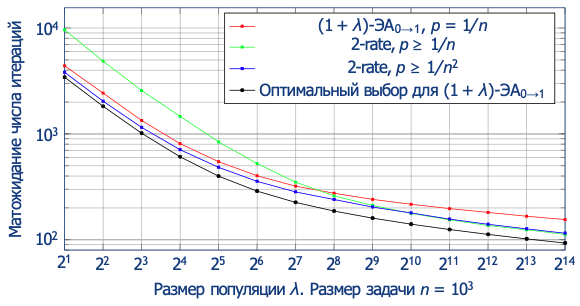
\includegraphics[width=0.8\linewidth]{images/c33_2rate.png}
    \caption{Пример}
    \label{fig:mpr}
\end{figure}
    